

\chapter{Einleitung}
\label{cha:Einleitung}
\dictum[Rainer Megerle (*1949), Chef Mergele AG, Nürnberg]{Es stimmt nicht, daß die Kosten die Preise bestimmen. Die im Markt erzielbaren Preise definieren die Kosten, die man sich leisten kann.}
 		
% -------------------------------------------------------------------------------------------------
% -------------------------------------------------------------------------------------------------
% -------------------------------------------------------------------------------------------------
\section{Motivation}

Das grundlegende Bestreben jedes Unternehmens ist es, seine Existenz am Markt zu sichern. Eine konjunkturell angespannte Wirtschaftslage, zunehmende Globalisierung der M\"arkte, zunehmender Konkurrenzdruck und kontinuierlich steigende
Anforderungen nach qualitativ hochwertigen Produkten stellen für die Unternehmen der Automobilindustrie wachsende Herausforderungen dar. 

Zus\"atzlich zu den oben genannten Faktoren erschwert ein Wechsel der Marktsituation die Situation der Unternehmen. In den 60er Jahren des vorigen Jahrhunderts \"uberstieg das Angebot der produzierenden Unternehmen bedingt durch den steigenden Wohlstand der Bev\"olkerung die Nachfrage. Es handelte sich um einen sogenannten Angebots- oder Verk\"aufermarkt. Diese Situation hat sich grunds\"atzlich ge\"andert. Auf den heutigen M\"arkten steht es dem Kunden frei, sich bei einer Vielzahl von global agierenden Unternehmen das f\"ur ihn passende Produkt auszusuchen. Der moderne Kunde erwartet dar\"uber hinaus ein auf seine individuelle Bed\"rfnisse angepasstes Produkt; es liegt eine sogenante Differenzierung der Nachfrage vor. Dies stellt an die Automobilhersteller die Anforderung, ihre Fahrzeuge in einer gro{\ss}en Konfigurierbarkeit und damit Variantenvielfalt anzubieten. 
 
\section{Kostenabsch\"atzung f\"ur CAD-Bauteile}

\subsection{Kostenabsch\"atzung f\"ur spritzgussgefertigte Bauteile}

\subsection{Dome}
\label{dome}



\subsection{Rippen}
Verst\"arkungsrippen sind ein wirksames Hilfsmittel, um die Steifigkeit und Festigkeit von Spritzgu{\ss}teilen zu erhöhen.
Der richtige Einsatz von Rippen kann Material und Gewicht einsparen, die Spritzzyklen verkürzen und dicke Querschnittbereiche vermeiden helfen, die beim Spritzgie{\ss}en zu Problemen führen könnten. Wenn Einfallstellen auf der einer Rippe
gegen\"uberliegenden Seite nicht akzeptabel sind, k\"onnen sie durch strukturierte Oberflächen oder andere geeignete Unterbrechungen im Bereich der Einfallstelle kaschiert werden.

\section{Das Projekt GoCart}
\label{goCart}

\subsection{H\"andisches Ausmessen von Domstrukturen}
\label{domeMeasure}

Das h\"andische Messverfahren zur Platzierung eines parametrischen Zylinders erfordert zun\"achst die Eingabe einer beliebigen Anzahl von Punkten auf der planaren Oberfl\"ache der Domstruktur. Hierf\"ur wurde grafisches Werkzeug entwickelt, das es dem Benutzer erlaubt, eine Reihe von dreidimensionalen Kugelobjekten durch Linksklick im 3D-Ansichtsfenster zu erzeugen. Die Koordinate der jeweiligen Kugel wird bestimmt, indem der 3D-Selektionsmechanismus (eng. \textit{Picking}) der Anwendung genutzt wurde, um den Schnittpunkt eines Strahls vom Klickpunkt im Ansichtsfenster auf eine Objektgeometrie zu bestimmen.

Diese Kugeln m\"ussen vom Benutzer kreisf\"ormig auf der Zylinderkappe angeordnet werden. Durch Rechtsklick kann dann ein interaktiver parametrischer Messzylinder, mit dem H\"ohe und Radius manipuliert werden kann, erzeugt werden. Das Zylinderobjekt ist an der Normalen der sogenannten \textit{Best-Fitting Plane} ausgerichtet. Eine \textit{Best-Fitting Plane} f\"ur eine dreidimensionale Punktemenge ist diejenige Ebene, die den aufsummierten orthogonalen Abstand der Punkte zur Ebene minimiert. Sie wird sowohl f\"ur die halbautomatische Erkennung von Domstrukturen als auch f\"ur die Segmentierung der Bauteile, die in Abschnitt \ref{cha:segment} beschrieben wird, verwendet. Im Rahmen der Masterarbeit wurde das bestehende, auf Singulärwertzerlegung basierende Verfahren, durch Hauptkomponentenanalyse ersetzt. Es wird im Abschnitt \ref{subsec:pca} näher beschrieben.

\begin{figure}[ht]
\centering
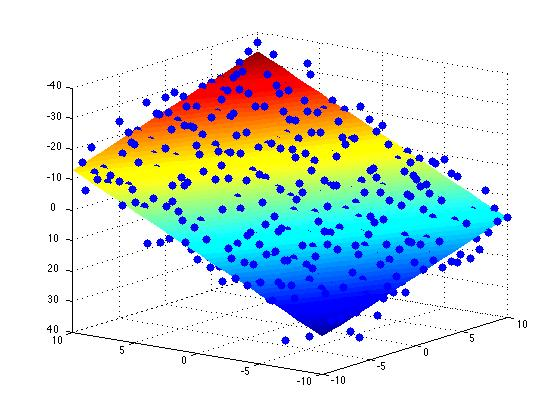
\includegraphics[width=10cm]{graphics/planefit.jpg}
\caption{H\"andische Erzeugung eines parametrischen Zylinders.}
\label{fig2}
\end{figure}

Der Zylinder kann so im Schwerpunkt der Punktwolke und an der Normalen der Best-Fitting Plane ausgerichtet erzeugt werden. Als voreingestellter Radius wird der Abstand des am weitesten zum Schwerpunkt entfernten Punktabstand genutzt.
Der Benutzer kann dann mit Hilfe eines Transformationsmanipulators die Höhe und den Radius weiter anpassen.

\subsection{H\"andisches Ausmessen von Rippenstrukturen}
\label{ribMeasure}

\section{Grundlagen der verwendeten computergrafischen Techniken}

Dreidimensionale Objekte k\"onnen in einem Rechner nur visualisiert und verarbeitet werden, wenn ihre Struktur durch ein geeignetes Modell beschrieben wird.

\subsection{B-Rep Geometrien}

Bei einem B-Rep Modell wird ein K\"orper durch die ihn begrenzenden Fl\"achen beschrieben.

\subsection{Triangulierte Geometrien}

Eine einfache M\"oglichkeit zur Repr\"sentation von geometrischen K\"orpern sind Dreiecksnetze, sogenannte Triangulierungen.

\subsection{Kollisonspr\"ufung}

In computergrafischen Systemen ist es oft erforderlich, den minimalen Abstand zwischen zwei geometrischen Objekten zu bestimmen. Um dies zu realisieren, sind effiziente Kollisionspr\"ufungsroutinen unbedingt notwendig. Unter
Kollisionspr\"ufung versteht man im Allgemeinen das Erkennen von Ber\"uhrungen
oder \"Uberlappungen zweier oder mehrerer geometrischer Objekte im zwei- oder dreidimensionalen Raum.
Ein geometrisches Objekt ist hier ein K\"orper, der durch ein Polygonnetz oder
ein Freiformfl\"achenmodell beschrieben werden kann.

Es existieren eine Reihe weiterer Anwendungen, f\"ur die eine effiziente Kollisions\-pr\"ufung
unbedingt erforderlich ist:

\begin{itemize}
	\item Beim {\em Virtual Prototyping} wird die Baubarkeit der transformierten
	Einzelkomponenten des Prototyps durch Kollisionstests gew\"ahrleistet
    \cite{zachmannThesis}.
	\item In der {\em Pfad- und Bewegungsplanung} gilt es, f\"ur einen Roboter mit
	beliebigen Freiheitsgraden einen Weg von einem Start- zu einem Zielpunkt zu
	finden, ohne das dieser mit Hindernissen kollidiert \cite{lavalle}.
	\item {\em Starrk\"orper-Physiksimulationen}  f\"uhren Kollisionspr\"ufung aus,
	um in jedem Zeitschritt der Simulation zu erfassen, ob ein dynamisches Objekt mit einem
	anderen Objekt der Szene kollidiert. So k\"onnen nat\"urliche
	Verhaltensweisen starrer K\"orper, wie beispielsweise das voneinander Abprallen
	von Billardkugeln, simuliert werden.
\end{itemize}

Diese Anwendungen stellen unterschiedliche Anforderungen an ein
Kollisionspr\"ufungssystem. Zum einen m\"ussen in k\"urzerster Zeit \"Uberlappungen
zwischen dynamischen Objekten erkannt werden, zum anderen muss eine
gro"se Menge Geometrie verarbeitbar sein. Ein einfacher Ansatz, die Kollisionen
einer Szene zu finden, ist, alle Dreiecke paarweise gegeneinaner
zu testen. Dies f\"uhrt jedoch (bei  {\em n}
Szenenobjekten) zu quadratischem Aufwand:

\begin{equation}
\frac{n*(n-1)}{2} \in \mathcal O(n^2)\label{quad}
\end{equation}

So sind keine echtzeitf\"ahigen \"Uberlappungstests realisierbar! Daher muss die
Berechnungzeit mit Hilfe von Optimierungsmethoden minimiert werden. Eine Idee,
den Aufwand zu reduzieren, ist, einen Divide-and-Conquer Ansatz zu verwenden \cite{Ericson05}. 

%Sogenannte "`{\em Zwei-Phasen Algorithmen}"' wenden so einen Divide-and-Conquer Ansatz folgenderma"sen an:
%Zun\"achst wird in der "`{\em weiten Phase}"' (eng. "`{\em Broad Phase}") versucht, Paare von Objekten zu 
%finden, die miteinander kollidieren k\"onnten, weil sie r\"aumlich benachbart sind. Eine exakte  Kollisionserkennung %ist dann in der "`{\em nahen Phase}"' (eng. "`{\em Narrow Phase}") nur noch zwischen diesen Objekten erforderlich.

\begin{figure}[H]
\centerline{
	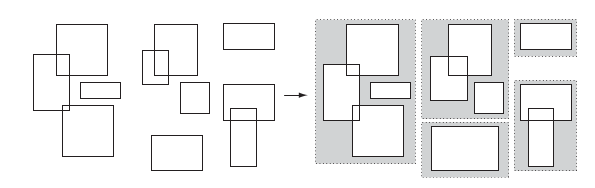
\includegraphics[width=0.7\columnwidth]{graphics/box.png}
}
\caption{Erkennung von disjunkten Objekten.}
\label{broadbox}
\end{figure}

In Abb. \ref{broadbox} sind auf der linken Seite um 11 Rechtecke auf Kollision zu pr\"ufen 55 Tests notwendig.
Nachdem in der "`weiten Phase"' 5 disjunkte Teilmengen erkannt wurden, kann die Anzahl der Tests in der "`nahen Phase"' auf 10 reduziert werden.

Ein Ansatz, die Anzahl der n\"otigen expliziten Dreiecks"-tests zu reduzieren, ist, anstelle der Dreiecke zun\"achst einen H\"ullk\"orper ({\em Bounding Volume}, kurz: {\em BV}) zu testen. Ein  H\"ullk\"orper ist ein
einfaches geometrisches Objekt wie beispielsweise ein W\"urfel oder eine Kugel, das das Objekt komplett
umh\"ullt. Die Idee ist, auszunutzen, dass die Schnitttests solcher K\"orper im Vergleich zu den eingeh\"ullten Objekten weniger aufwendig sind. So k\"onnen zun\"achst die Bounding Volumes zweier Objekte auf Kollision
getest\-et werden und nur dann, wenn dieser Schnitttest positiv verl\"auft, muss
die Dreiecksmenge der Objekte in der "`nahen Phase"' explizit gepr\"uft werden.

Die Nutzung von H\"ullk\"orpern reduziert den quadratischen Aufwand der Kollisionsp\"ufung einer Szene mit {\em n} Dreiecken soweit um einen konstanten Faktor {\em k}:
\begin{equation}
\forall k \in [0,1]:
k* \frac{n*(n-1)}{2} 
\in \mathcal O(n^2)
\end{equation}
Obwohl hierdurch der Rechenaufwand signifikant verringert werden kann, verbessert dies die Komplexit\"atsklasse des naiven Ansatzes nicht; die Anzahl der n\"otigen paarweisen Schnitttests zwischen den H\"ullen w\"achst noch immer
quadratisch bez\"uglich der Anzahl der Szenenobjekte.

Eine M\"oglichkeit, den Aufwand weiter zu reduzieren, ist die Nutzung von Hierachien aus H\"ullk\"orpern (sogenannten {\em Bounding Volume Hierachien} oder {\em BVH}). Dieser Ansatz wurde 1996 in dem Artikel "`{\em OBBTree: A Hierarchical Structure for Rapid Interference Detection}"' vorgestellt und hat seit dem die Forschung an Kollisionspr\"ufungsalgorithmen stark beeinflu"st \cite{Gottschalk}. BVH's betten die H\"ullk\"orper der Objekte rekursiv in gr\"o"sere BV's ein und ordnen diese in einer Baumstruktur an. So kann die Zeitkomplexit\"at des Algorithmus auf logarithmischen Aufwand verringert werden. Abbildung \ref{bvh} zeigt eine Hierachie weltachsenorientierter H\"ullquader, mit der f\"unf Objekte eingeh\"ullt werden.

\begin{figure}[H]
\centerline{
	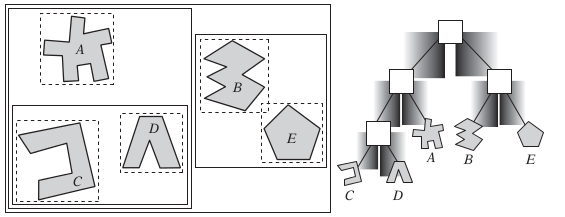
\includegraphics[scale=0.60]{graphics/bvh.png}
}
\caption{Bounding Volume Hierachie aus 5 Objekten. Auf der linken Seite wird
die Szene rekursiv umh\"ullt so dass die Baumstruktur auf der rechten Seite
daraus resultiert. }
\label{bvh}
\end{figure}

Der Ansatz rekursive H\"ullk\"orper in einer Baumstruktur anzuordnen, l\"asst
sich auch auf die Dreieckesmenge eines Objektes ausweiten. Hierbei wird die
Dreiecksmenge eines Objektes als Punktewolke interpretiert, die dann mittels
Top-Down Ans\"atzen so lange weiter unterteilt wird, bis ein Abbruchkriterium
erreicht ist. Abbildung \ref{bvho} zeigt eine solche Hierachie aus AABB's \"uber
der Dreiecksmenge eines Objektes.

\begin{figure}[H]
\centerline{
	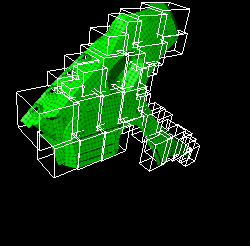
\includegraphics[scale=0.7]{graphics/BV-Hierarchie5.png}
}
\caption{Bounding Volume Hierachie \"uber den Dreiecken eines Objektes.}
\label{bvho}
\end{figure}

Um eine Szene, f\"ur die eine H\"ullk\"orperhierachie erzeugt wurde, auf Kollision zu testen, mu"s die Hierachie traversiert werden. Auf jeder Baumebene, die w\"ahrend der Traversierung besucht wird,  werden die BV's der Knoten
gegeneinander auf Kollision gepr\"uft. Wenn eine \"Uberschneidung zwischen zwei Bounding Volumes gefunden wurden, wird
die Baumsuche in diesen \"Asten fortgesetzt. Auf diese Weise wird rekursiv bis in die Blattknoten vorgegangen. Sollten die H\"ullen zweier Blattknoten \"uberlappen, kann eine Kollision zwischen den eingeh\"ullten Dreiecken bestehen, die dann in der "`Narrow Phase"' aufzul\"osen ist.




Im Rahmen dieser Arbeit wurde eine properit\"are Implementierung der frei verf\"ugbaren Bibliothek Proximity Query
Package (PQP) verwendet \cite{PQP}.


\subsection{3D-Selektion}


\section{Aufgabenstellung}
\label{problem}

\section{Aufbau der Arbeit}

